\documentclass[../rapport_MVEX01-11-05]{subfiles}
\begin{document}

\section{Klassificering av hudfärg och urskiljning av händer}
Både vår sannolikhetsfördelning för icke-hudfärg och motsvarande
fördelning från \citeasnoun{Elmezain08} har väldigt liten varians,
dvs diagonalelement i kovariansmatrisen. För att ge en bra
hudidentifiering bör denna varians vara stor, annars klassas allt
''bortom'' hudfärg (rödaktiga färger) som hud. Vi valde därför att
istället sätta variansen oändlig, så att sannolikhetsfördelningen för
bildpunkter som inte föreställde hud var likformig.

Den sannolikhetsfördelning vi fick fram genom egen bildanalys skiljde
ut händer relativt bra, men den lämnade ett antal hål i handen. Även
den fördelning som ges av \citeasnoun{Elmezain08} fungerade bra, och
gav färre falska bildpunkter med icke-hud. Denna fördelning var därför den som
användes i resten av arbetet. \notes{Bör detta vara metod istället?}

Metoden för identifiering av händer visade sig fungera mycket väl i
kontrollerad miljö. De krav som ställdes var, förutom långärmad
tröja, att belysningen skulle vara god och helst komma från lysrör
samt att bilden inte fick innehålla för stora rödfärgade partier --- detta
då vårt hudfärgsområde var för stort åt det röda hållet. 

En visualisering av hudurskiljningen kan ses i figur
\ref{fig:hudklassificering}, där alla områden som klassats som hud
gjorts vita och övriga svarta. Handen är markerad med en inneslutande
låda i figur \ref{fig:boundingbox}.

\begin{figure}
  \centering
  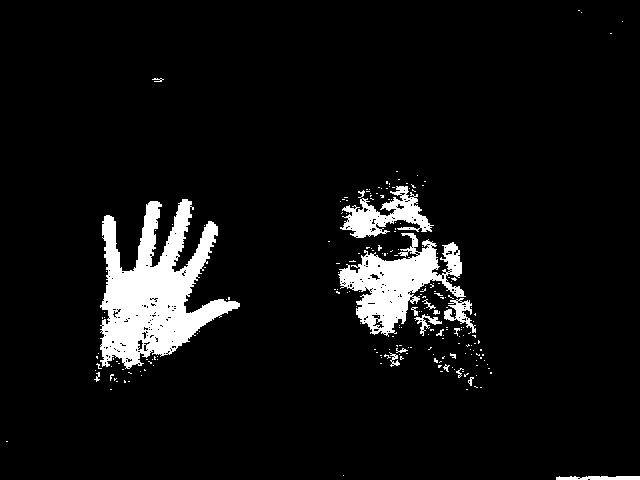
\includegraphics[width=0.8\columnwidth]{bilder/whiteskin}
  \caption{Figuren visar de områden i bilden som klassats som hud.
  Observera det vita bruset i bildens kanter, vilket filtreras bort med
  morfologiska operationer.}
  \label{fig:hudklassificering}
\end{figure}

\begin{figure}
  \centering
  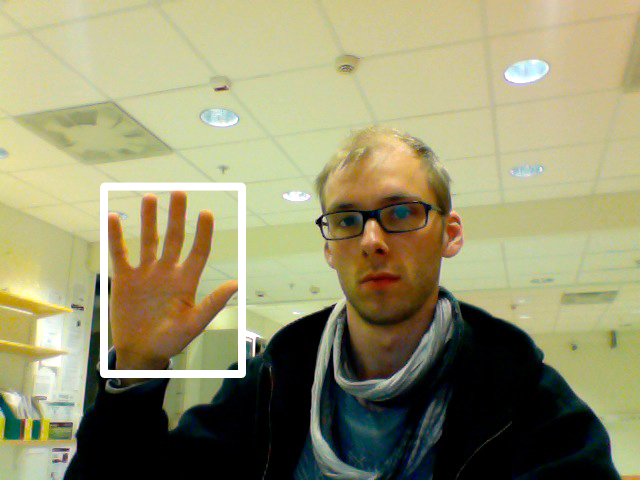
\includegraphics[width=0.8\columnwidth]{bilder/boundingbox}
  \caption{Handen har ringats in av programmet, som det
  ''tillräckligt'' stora objekt som befinner sig
  längst till vänster i bilden.}
  \label{fig:boundingbox}
\end{figure}

\end{document}
